\def \sectionauthors {Dennis Köb}
\subsection{Anforderungen}
Das Ziel der Fahrzeugerkennung ist es Fahrzeuge auf mehrere Parklücken eines Parkplatzes zu erkennen. Die daraus 
gewonnen Zustände sollen an das Webinterface übermittelt und an den jeweilige Parklücken über LEDs ausgegeben werden. 
\subsection{Vorstudie}

\subsection{Erkennung von Metallen über Spulen}
Grundsätzlich werden in der Realität häufig Spulen verwendet, welche unter dem Asphalt verbaut sind, um darüberliegende
Fahrzeuge zu detektieren. Als Messprinzip wird die Änderung des magnetischen Widerstands $R_{m}$ bei konstanter magnetischer Spannung $U_{m}$ und
daraus resultierende magnetischen Fluss $\phi$
Es gelten für diese Größen der folgende Zusammenhänge:

\begin{equation} \label{eq:phi}
    \phi = \frac{U_{m}}{R_{m}}
\end{equation}

Wobei \\
$\phi$ = magnetischer Fluss \\
$R_{m}$ = magnetischer Widerstand \\
$U_{m}$ = magnetische Spannung
\pagebreak

Der magnetische Widerstand lässt sich wiederum durch die Eigneschaften der Spule bestimmen. Die Formel hierfür lautet:

\begin{equation} \label{eq:Rm}
    R_{m} = \frac{N \cdot (2a + 2b)}{\mu_{0} \cdot \mu_{r} \cdot A} 
\end{equation}


Wobei \\
\begin{equation} \label{eq:A}
    A = a \cdot b
\end{equation}
$N$ = Anzahl der Windungen der Spule \\
$a$ = Breite der Spule in m \\
$b$ = Länge der Spule in m\\
$\mu_{0}$ = \SI[per-mode = symbol]{1.2566e-6}{\newton\per\ampere\squared} = magnetische Feldkonstante \\
$\mu_{r}$ = relative Permeabilität  \\
$A$ = Fläche der Spule

Bis auf die relative Permeabilität sind alle alle anderen Variablen konstant. Daraus lässt sich schlussfolgern, dass der magnetische
Fluss $\phi$ anhand der Gleichung \ref{eq:phi} und \ref{eq:Rm} proportional zur relativen Permeabilität ist. 

\begin{equation} \label{iq:phi}
    \phi \propto \mu_{r}
\end{equation}
Der Fluss $\phi$ hängt somit auch von den Materialien ab durch die er fließt. In der nächsten Abbildung kann man erkennen,
wie ein Fahrzeug über eine im Boden installierte Spule den magnetischen Fluss $\phi$ und somit die magnetische Flussdichte $B$
beeinflussen kann. 
\begin{figure}[H]
    \centering
    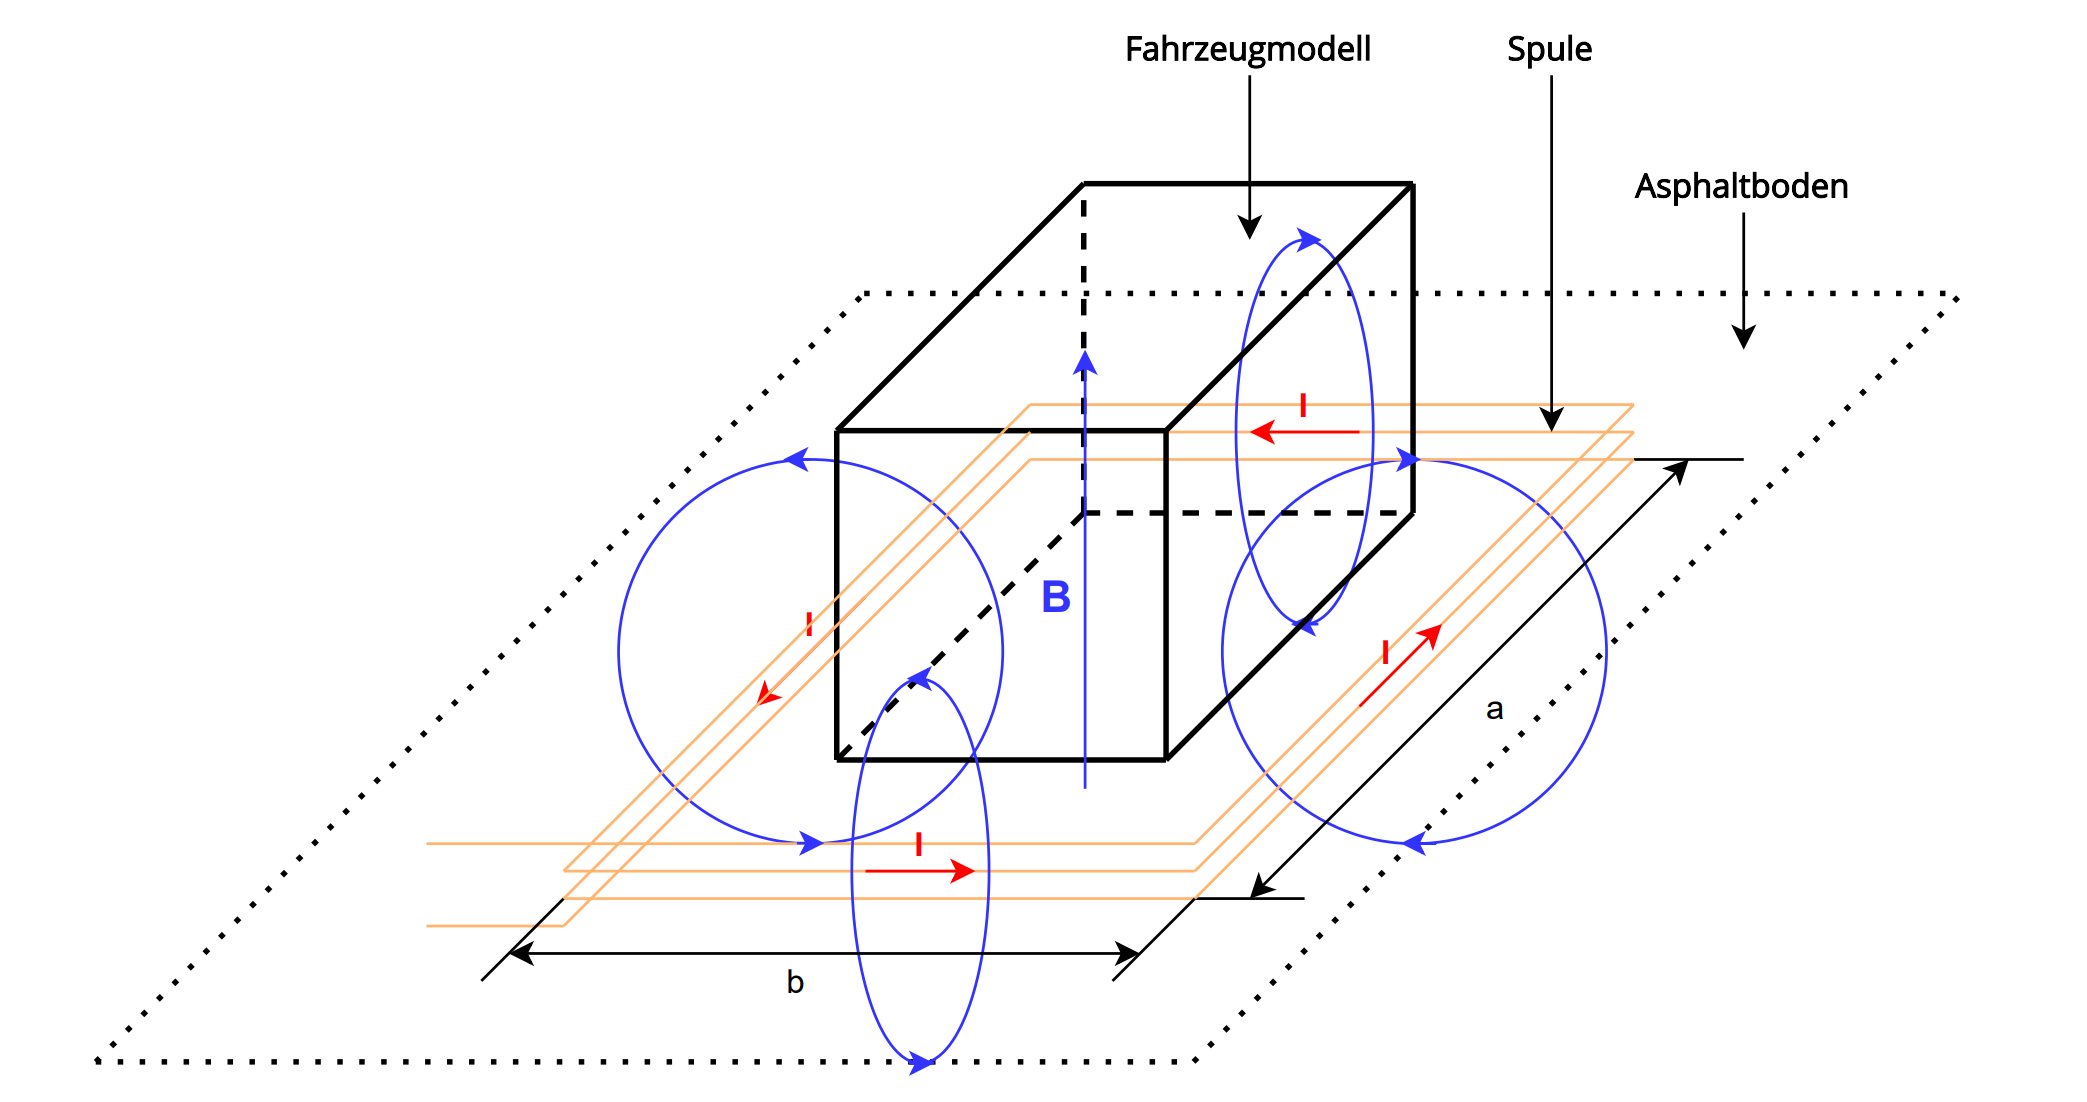
\includegraphics[width=1\linewidth]{fahrzeugerkennung/Spuleninstallation.png}
    \caption{Installation der Spule}
  \end{figure}
Um diese Größen auslesbar zu machen, müssen diese magnetischen bei einer direkten Messung in elektrische Größen umgewandelt
werden.
Hierfür geltzen folgende Zusammenhänge:

\begin{equation} \label{eq:L_phi}
    L = \frac{N \cdot \phi}{I} = \frac{\psi}{I} 
\end{equation}
Wobei \\
$L$ = Induktivität der Spule \\
$I$ = Strom der durch die Spule fließt \\
$N$ = Anzahl der Windungen der Spule \\
$\psi$ = Verkettete Fluss

\pagebreak
\begin{equation} \label{eq:L_i}
    u(t) = L * \frac{di(t)}{dt}
\end{equation}

Wobei \\
$L$ = Induktivität der Spule \\
$i(t)$ = Strom der durch die Spule fließt zum Zeitpunkt t \\
$u(t)$ = Spannung die an der Spule anliegt zum Zeitpunkt t \\

So lässt sich bei Bekanntheit von Strom und Spannung auf die Induktivität und mit der Gleichung \ref{eq:L_phi} 
und mit den Zusammenhang \ref{iq:phi} auf die magnetischen Eigenschaften des Materials rückschließen. 
Diese Art der Detektion bietet viele praktische Vorteile.

\begin{itemize}
    \item \textbf{Größerer Messbereich} \\
    Im Vergleich zu anderen Detektionsmethoden wie einer Leichtschranke kann man einen größeren Bereich durch die Wirkfläche
    der Spule abdecken. So lassen sich auch kleinere Kraftfahrzeuge wie Motorräder oder Mopeds besser erkennen.
    \item \textbf{Schutz vor Umweltfaktoren} \\
    Durch den Verbau im Boden ist die Messeinrichtung vor Umwelteinflüssen wie Regen, Frost, hohen beziehungsweise
    niedrigen Temperaturen und Korrosion besser geschütz. Dies verringert auch den Einfluss dieser Störfaktoren auf die Eigenschaften
    Spule und somit auf die daraus resultierenden Messergebnisse.
    \item \textbf{Ausschließung von Materialien} \\
    Alle nicht metallische Stoffe werden von diesem Messprinzip nicht wahrgenommen. So können Verschmutzungen wie Blätter und Staub, welche
    visuelle Sensoren stören können, die Detektion nicht behindern.
    
\end{itemize}
\subsubsection{Messung der ferromagnetischer Metalle}
Bei ferromagnetischen Metalle ist die Permeabilitätszahl  $\mu_{r}$ sehr viel größer 1. Dies bedeutet, dass eine 
\paragraph{RL-Oszillator mit Timer Baustein}
\paragraph{Puls-Ladung mit Mikrokontroller}
\subsubsection{Messung paramagnetischer Metalle}
\paragraph{Messung eines Wechselstromes}
\paragraph{Messung der Resonanzfrequenz eines Oszillastors}

\subsection{RS485 Bussystem}
\subsubsection{Überblick}
\subsubsection{Elektrische Spezifikation}
\subsubsection{Implementation eines eigenen Protokolls}

\subsection{Mikrokontroller Slave-Geräte}
\subsubsection{Überblick}
\subsubsection{Atmega328PB}
\subsubsection{Peripherie des Mikrokontrollers}
\paragraph{Spannungswandler}
\paragraph{RS485 Pegelwandler}
\paragraph{Digitale Ein- und Ausgänge}
\subsubsection{Layout des Slave-Gerätes}
\subsubsection{Gehäuse}


\subsection{USB-Master}
\subsubsection{USB-Bussadapter Gerät}
\paragraph{Überblick}
\paragraph{FT232RL}
\paragraph{Spannungsversorgung}
\paragraph{USB-C Anschluss}
\paragraph{Layout des Master-Geräts}
\paragraph{Gehäuse}

\subsubsection{Master Programm}
\paragraph{Benötigte Software}
\paragraph{Adressvergabe}
\paragraph{Frequenzauslesung}

\paragraph{Auswertung}
\paragraph{API-Post}

\subsubsection{RaspberryPi als Mastergerät}
\paragraph{SSH Remote Zugriff}
\paragraph{Code Deployment}
\paragraph{Unittest}

\pagebreak


